\documentclass[xcolor=dvipsnames,table]{beamer}

\usepackage{latexsym}
\usepackage[utf8]{inputenc}
\usepackage[brazil]{babel}
\usepackage{amssymb}
\usepackage{amsmath}
\usepackage{stmaryrd}
\usepackage{fancybox}
\usepackage{datetime}
\usepackage[T1]{fontenc}
\usepackage{graphicx}
\usepackage{graphics}
\usepackage{url}
\usepackage{algorithmic}
\usepackage{algorithm}
\usepackage{acronym}
\usepackage{array}

\newtheorem{definicao}{Definio}
\newcommand{\tab}{\hspace*{2em}}

\mode<presentation>
{
  \definecolor{colortexto}{RGB}{0,0,0}
 
  \setbeamertemplate{background canvas}[vertical shading][ bottom=white!10,top=white!10]
  \setbeamercolor{normal text}{fg=colortexto} 

  \usetheme{Warsaw}
}

\title{Problema da Parada e \\Linguagens Turing-irreconhecíveis} 

\author{
  Esdras Lins Bispo Jr. \\ \url{bispojr@ufg.br}
  } 
 \institute{
  Teoria da Computação \\Bacharelado em Ciência da Computação}
\date{\textbf{06 de julho de 2017} }

\logo{
\includegraphics[width=1cm]{images/ufgJataiLogo.png}}

\begin{document}

	\begin{frame}
		\titlepage
	\end{frame}

	\AtBeginSection{
		\begin{frame}{Sumário}%[allowframebreaks]{Sumário}
    		\tableofcontents[currentsection]
    		%\tableofcontents[currentsection, hideothersubsections]
		\end{frame}
	}

	\begin{frame}{Plano de Aula}
		\tableofcontents
		%\tableofcontents[hideallsubsections]
	\end{frame}
    
    \section{Revisão}
	
	\subsection{Conjunto Incontáveis}

	\begin{frame}{Conjuntos Incontáveis}
		\begin{block}{Teorema 4.17}
			$\mathbb{R}$ é incontável.
		\end{block} 
		\begin{block}{Ideia da Prova}
			\begin{itemize}
				\item De forma a mostrar que $\mathbb{R}$ é incontável, mostramos que nenhuma correspondência existe entre $\mathbb{N}$ e $\mathbb{R}$.
				\begin{itemize}
					\item Supomos, a princípio, que a correspondência $f$ existe.
					\item Logo após, apresentamos um valor $x \in \mathbb{R}$ que não está emparelhado com valor algum em $\mathbb{N}$ \\(o que indica um absurdo).				
				\end{itemize}
			\end{itemize}
		\end{block}
	\end{frame}
	
	\begin{frame}{Conjuntos Incontáveis}
		\begin{center}
			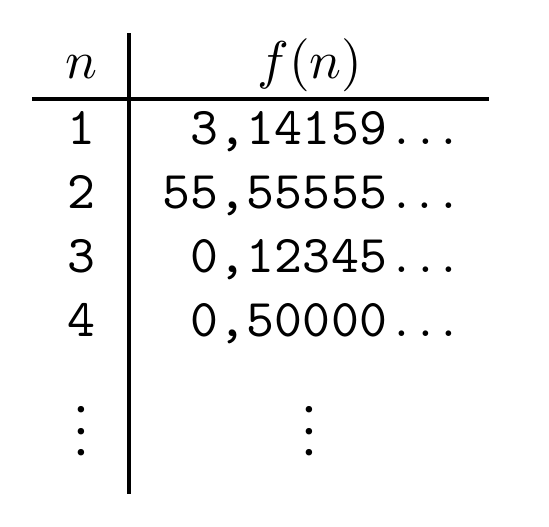
\includegraphics[width=6cm]{images/fHip.png}
			
			{\bf Figura:} Suposta correspondência $f$ entre $\mathbb{N}$ e $\mathbb{R}$.
		\end{center}
	\end{frame}
	
	\begin{frame}{Conjuntos Incontáveis}
		\begin{center}
			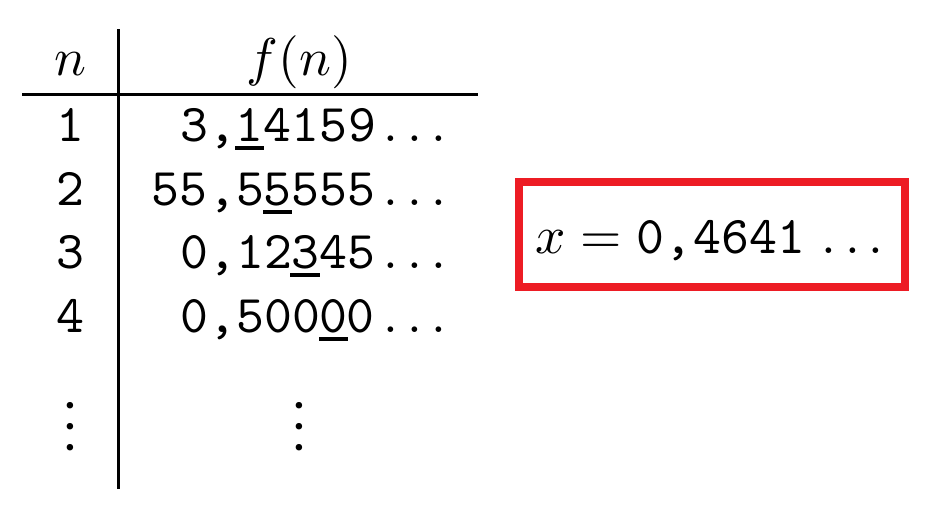
\includegraphics[width=9cm]{images/fHipX.png}
			
			{\bf Figura:} Construção de $x$ a partir da correspondência $f$.
		\end{center}
	\end{frame}
	
	\begin{frame}{Conjuntos Incontáveis}
		\begin{block}{Considerações}
			Apenas deve-se ter o cuidado de escolher dígitos para $x$ \\diferentes de 0 e 9, devido ao fato de 
			\begin{center}
				$3,999 \ldots = 4,000 \ldots$
			\end{center}
		\end{block}
	\end{frame}
	
	\begin{frame}{Conjuntos Incontáveis}
		\begin{exampleblock}{Corolário do Teorema 4.17}
			Algumas linguagens não são Turing-reconhecíveis.
		\end{exampleblock}
		\begin{block}{Ideia da Prova}
			\begin{enumerate}
				\item Observar que o conjunto de todas as máquinas de Turing é contável;
				\item Observar que o conjunto de todas as linguagens é incontável.
				\item Como há mais linguagens do que máquinas de Turing, então algumas linguagens não podem ser Turing-reconhecíveis.
			\end{enumerate}
		\end{block}
	\end{frame}
	
	\begin{frame}{Conjuntos Incontáveis}
		\begin{block}{O conjunto de todas as máquinas de Turing é contável}
			\begin{itemize}
				\item $\Sigma^*$ é contável; 
				\item Cada máquina de Turing pode ser codificada em uma cadeia $\langle M \rangle$;
				\item O conjunto $C$ de todas as máquinas de Turing pode ser representado por um conjunto de cadeias $\langle M \rangle$; 
				\item É possível enumerar $C$;
				\item Logo $C$ é contável.
			\end{itemize}
		\end{block}
	\end{frame}

	\begin{frame}{Conjuntos Incontáveis}
		\begin{center}
			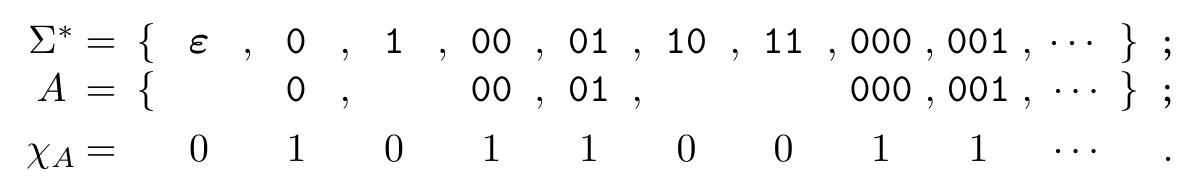
\includegraphics[width=11cm]{images/seqCar.png}
			
			{\bf Figura:} Construção de $\mathcal{X}A$ a partir da correspondência $\Sigma^*$.
		\end{center}
	\end{frame}
	
	\begin{frame}{Conjuntos Incontáveis}
		\begin{block}{O conjunto de todas as linguagens é incontável}
			\begin{itemize}
				\item O conjunto $B$ de todas as sequências binárias infinitas é incontável;
				\item Qualquer linguagem pode ser descrita como uma sequência característica;
				\item O conjunto $L$ de todas as linguagens podem ser representado por um conjunto de sequências \pause característica; 
				\item A função $f : L \rightarrow B$ \\(em que $f(A)$ é igual à sequência característica de $A$) \\é uma correspondência;
				\item Logo, como $B$ é incontável, $L$ é incontável.
			\end{itemize}
		\end{block}
	\end{frame}

	\section{Problema da Parada}
	\begin{frame}{Problema da Parada}
		\begin{block}{$A_{MT}$ é indecidível (Ideia da prova)}
			\begin{itemize}
				\item Vamos supor que $H$ decida $A_{MT}$ \pause
				\item Vamos construir a MT $D$ conforme a descrição abaixo:\\ \pause
				$D$ = ``Sobre a entrada $\langle M \rangle$, em que $M$ é uma MT:
				\begin{enumerate}
					\item Rode $H$ sobre a entrada $\langle M, \langle M \rangle \rangle$.
					\item Dê como saída o oposto do que $H$ dá como saída; ou seja, se $H$ aceita, {\it rejeite} e se $H$ rejeita, {\it aceite}.''
				\end{enumerate} \pause
				\item Entretanto, $D(\langle D \rangle)$ leva a uma contradição. \pause
				\item Logo, $A_{MT}$ é indecidível.
			\end{itemize}
		\end{block}
	\end{frame}

	\begin{frame}{Problema da Parada}
		\begin{block}{$A_{MT}$ é indecidível (Ideia da prova)}
			Resumindo... \pause
			\begin{itemize}
				\item $H$ aceita $\langle M, \omega \rangle$ exatamente quando $M$ aceita $\omega$. \pause
				\item $D$ rejeita $\langle M \rangle$ exatamente quando $M$ aceita $\langle M \rangle$. \pause
				\item $D$ rejeita $\langle D \rangle$ exatamente quando $D$ aceita $\langle D \rangle$ ({\color{red} Absurdo!!!}).
			\end{itemize}
		\end{block}
	\end{frame}

	\begin{frame}{Problema da Parada}
		\begin{center}
			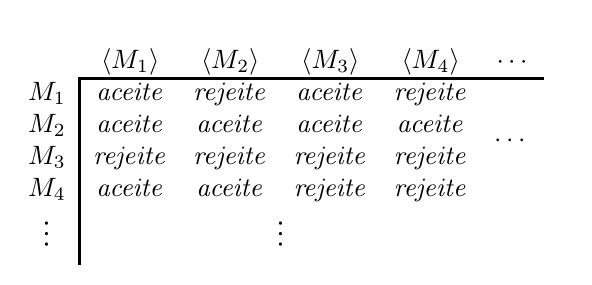
\includegraphics[width=11cm]{images/h.png}
			
			 A entrada $i,j$ é o valor de $H$ sobre a entrada $\langle M_i , \langle M_j \rangle \rangle$.
		\end{center}
	\end{frame}

	\begin{frame}{Problema da Parada}
		\begin{center}
			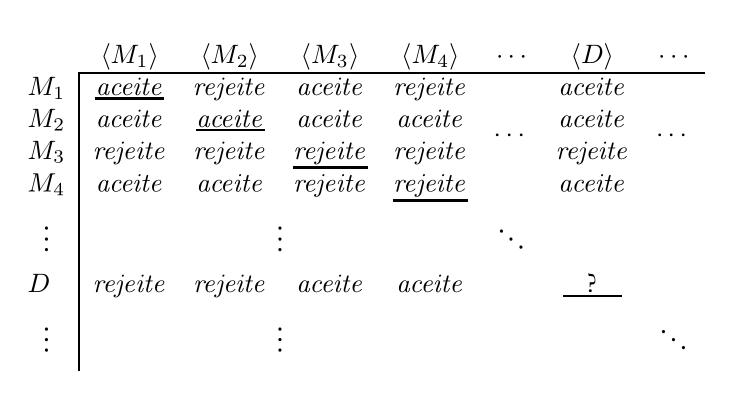
\includegraphics[width=11cm]{images/d.png}
			
			{\bf Figura:} Se D estiver na figura, uma contradição ocorre em ``?''.
		\end{center}
	\end{frame}

	\section{Linguagem Turing-Irreconhecíveis}
	\begin{frame}{Linguagens Turing-irreconhecíveis}
		\begin{block}{Teorema 4.22}
			Uma linguagem é decidível sse ela é Turing-reconhecível e co-Turing-reconhecível.
		\end{block} \pause
		\begin{block}{Corolário 4.23}
			$\overline{A_{MT}}$ não é Turing-reconhecível.
		\end{block}
	\end{frame}
	
	\begin{frame}
		\titlepage
	\end{frame}
	
\end{document}